	\begin{figure}[!thpb]
		\centering
		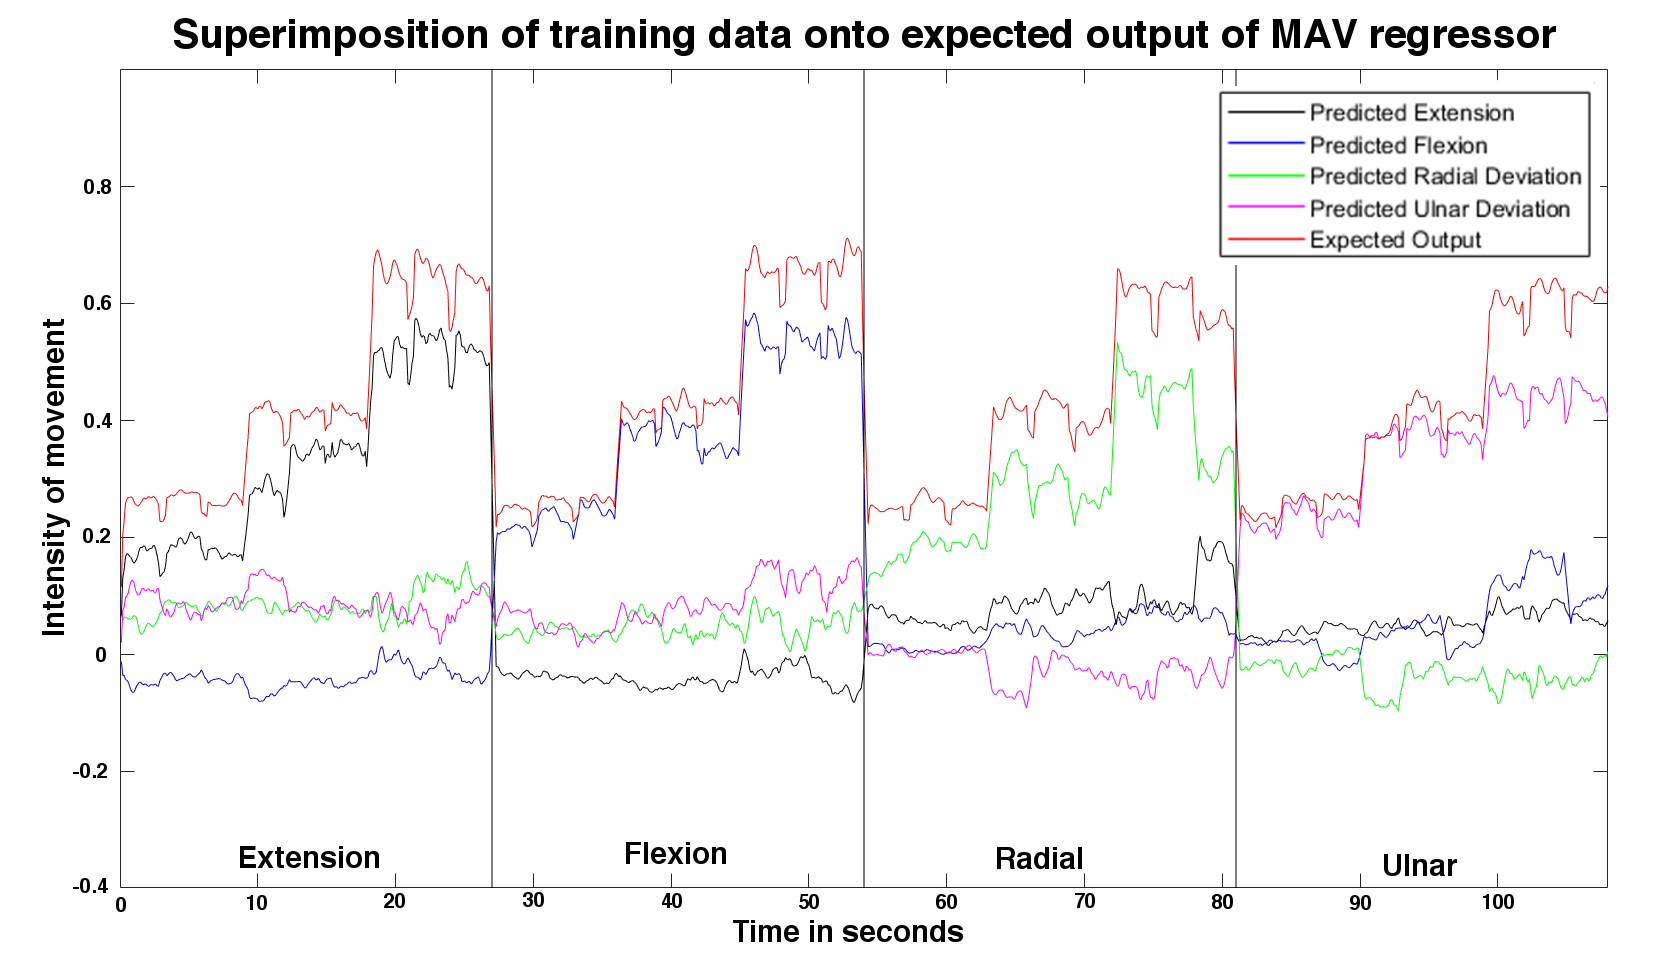
\includegraphics[width=0.4\textwidth]{figures/NewSuperPositionTestDataMAV}  %<--but is not needed.
		\caption{Plot of the actual data, red plot, superimposed on the output of the regressors trained with the MAV features. The plot is divided into four segments, where each segment shows a different movement performed. Each segment has the same sample size.}
		\label{fig:SuperPositionTrainingMAV}  %<--give the figure a label, so you can reference!
	\end{figure}
	
	\begin{figure}[!thpb]
		\centering
		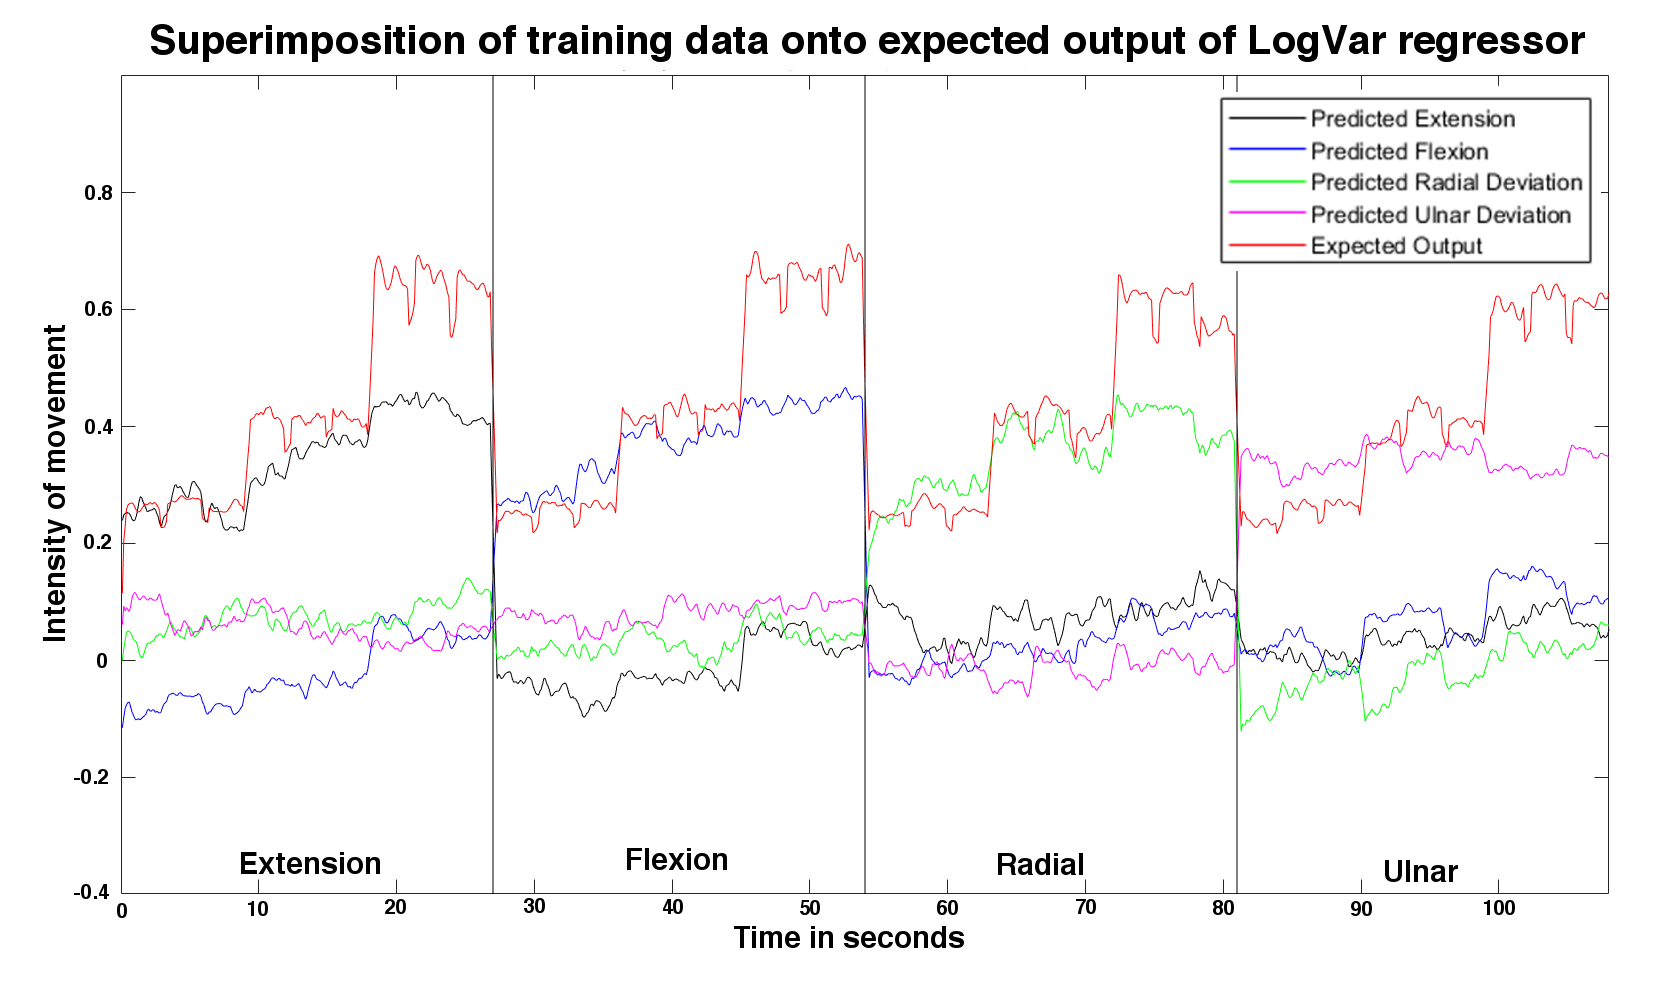
\includegraphics[width=0.4\textwidth]{figures/NewSuperPositionTestDataLogVar}  %<--but is not needed.
		\caption{Plot of the actual data, red plot, superimposed on the output of the regressors trained with the LogVar features. The plot is divided into four segments, where each segment shows a different movement performed. Each segment has the same sample size.}
		\label{fig:SuperPositionTrainingLogVar}  %<--give the figure a label, so you can reference!
	\end{figure}
	
	\begin{table}[!thpb]
		\begin{center}
			\begin{tabular}{l l l}
				\hline
				\textbf{Feature} & \textbf{Overall mean error} & \textbf{Standard deviation}\\
				\hline
				Extension & 0.1030 & $\pm 0.0210$ \\
				Flexion & 0.1102 & $\pm 0.0296$ \\
				Radial Deviation & 0.1206 & $\pm 0.0298$ \\
				Ulnar Deviation & 0.1143 & $\pm 0.0334$ \\
				Overall & 0.1059 & $\pm 0.0306$ \\
				\hline
			\end{tabular}
			\caption{RMSE for the implemented MAV regressor}
		\end{center}
	\end{table}
	
	\begin{table}[!thpb]
		\begin{center}
			\begin{tabular}{l l l}
				\hline
				\textbf{Feature} & \textbf{Overall mean error} & \textbf{Standard deviation}\\
				\hline
				Extension & 0.1157 & $\pm 0.0469$ \\
				Flexion & 0.1102 & $\pm 0.0241$ \\
				Radial Deviation & 0.1142 & $\pm 0.0256$ \\
				Ulnar Deviation & 0.1312 & $\pm 0.0310$ \\
				Overall & 0.1178 & $\pm 0.0272$ \\
				\hline
			\end{tabular}
			\caption{RMSE for the implemented LogVar regressor}
		\end{center}
	\end{table}
	
	\begin{table}[!thpb]
		\begin{center}
			\begin{tabular}{l l l}
				\hline
				\textbf{Feature} & \textbf{Overall mean error} & \textbf{Standard deviation}\\
				\hline
				Extension & 0.1646 & $\pm 0.0753$ \\
				Flexion & 0.1391 & $\pm 0.0841$ \\
				Radial Deviation & 0.2018 & $\pm 0.0424$ \\
				Ulnar Deviation & 0.1743 & $\pm 0.0905$ \\
				Overall & 0.1700 & $\pm 0.0759$ \\
				\hline
			\end{tabular}
			\caption{RMSE for the implemented MAV regressor}
		\end{center}
	\end{table}
	
	The overall mean of the RMSE of MAV is 0.0943 with a standard deviation of $\pm 0.0290$, where the highest mean of a regressor is 0.1088 and the highest standard deviation is $\pm 0.0366$. The overall mean of the RMSE of LogVar is 0.1107 with a standard deviation of $\pm 0.0298$, where the highest mean of a regressor is 0.1216 and the highest standard deviation is $\pm 0.0402$. MAV appears to yield a lower mean RMSE and a lower standard deviation than LogVar - both with the overall RMSE and for the movement with the highest RMSE.
	
	\begin{table}[!thpb]
		\begin{center}
			\begin{tabular}{l l l}
				\hline
				\textbf{Feature} & \textbf{Overall mean error} & \textbf{Standard deviation}\\
				\hline
				Extension & 0.1552 & $\pm 0.0514$ \\
				Flexion & 0.1680 & $\pm 0.0508$ \\
				Radial Deviation & 0.1681 & $\pm 0.0540$ \\
				Ulnar Deviation & 0.2078 & $\pm 0.0621$ \\
				Overall & 0.1748 & $\pm 0.0563$ \\
				\hline
			\end{tabular}
			\caption{RMSE for the implemented LogVar regressor}
		\end{center}
	\end{table}
	
	\begin{table}[!thpb]
		\begin{center}
			\begin{tabular}{l l}
				\hline
				\textbf{Compared features} & \textbf{P-Value}\\
				\hline
				LogVar, MAV & 0.0044 \\
				LogVar test data, MAV test data & 0.1138 \\
				LogVar test data, LogVar & 0.0001 \\
				MAV test data, MAV & 0.000002 \\
				\hline
			\end{tabular}
			\caption{P-Values for comparison of the features}
		\end{center}
	\end{table}
	It was found that the P-value of a Friedman's statistical test showed a significant difference (p = 0.0044) between the RMSE for the MAV and LogVar regressors with the training data as input, where LogVar has the higher mean. When examining the RMSE for the regressors with unknown test data consisting of 50\% contractions of all movements in all limb positions, it was shown that there is no significant difference (p = 0.1138) between the offline performance of the two regressors. When comparing the offline tests with training data and 50\% test data, it was shown that there's a significant difference for both LogVar (p = 0.000002) and LogVar (p = 0.0001), where the mean is higher for the unknown 50\% data in both cases.
	
	\begin{figure}[!thpb]
		\centering
		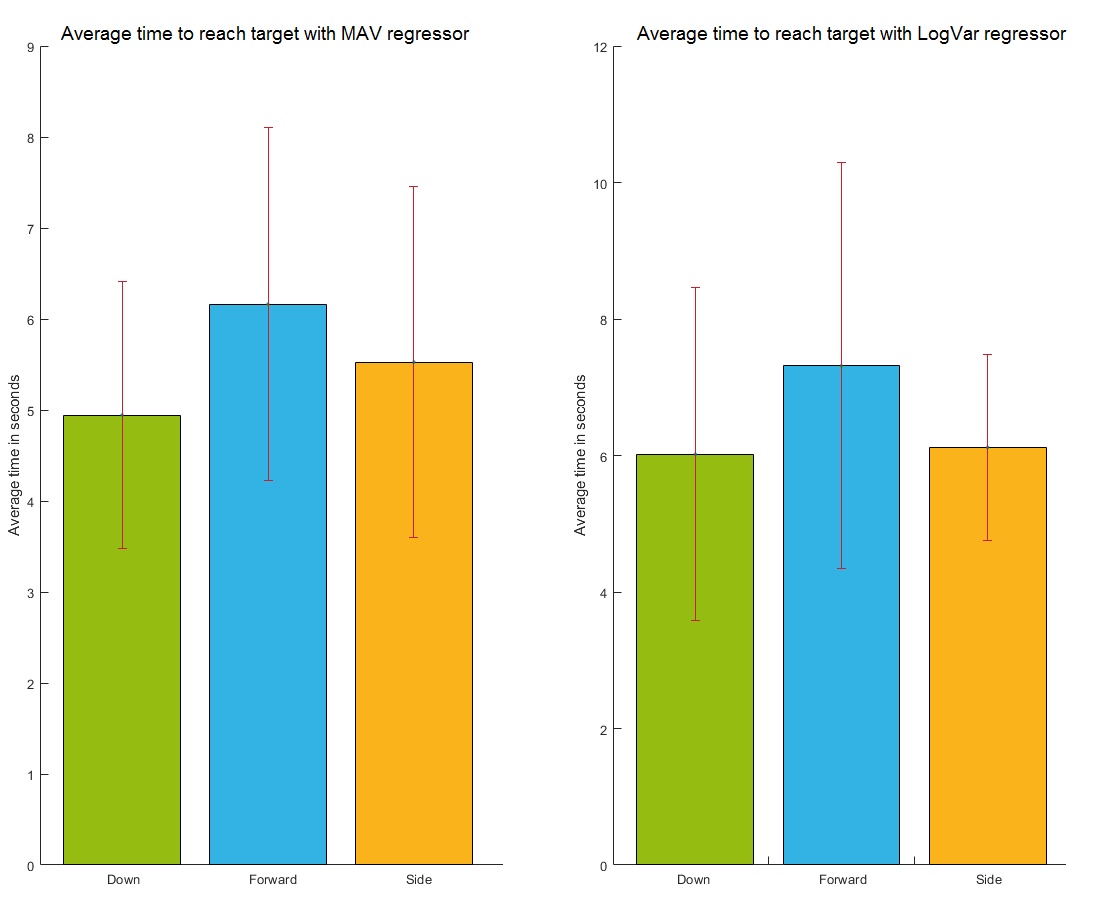
\includegraphics[width=0.4\textwidth]{figures/GotItTime}  %<--but is not needed.
		\caption{Plot of the actual data, red plot, superimposed on the output of the regressors trained with the MAV features. The plot is divided into four segments, where each segment shows a different movement performed. Each segment has the same sample size.}
		\label{fig:GotItTime}  %<--give the figure a label, so you can reference!
	\end{figure}
	
	\begin{table}![thpb]
		\begin{center}
			\begin{tabular}{l l l}
				\hline
				\textbf{Limb position, feature} & \textbf{Overall mean error} & \textbf{Standard deviation}\\
				\hline
				Down, MAV & 5.3377 & $\pm 1.5696$ \\
				Forward, MAV & 8.1791 & $\pm 4.7145$ \\
				Side, MAV & 6.0490 & $\pm 2.0490$ \\
				Down, LogVar & 6.5404 & $\pm 2.5315$ \\
				Forward, LogVar & 7.9123 & $\pm 3.4572$ \\
				Side, LogVar & 6.9325 & $\pm 2.3036$ \\
				\hline
			\end{tabular}
			\caption{Test scores for the different limb for MAV and LogVar regressors}
		\end{center}
	\end{table}
	\begin{table}[!thpb]
		\begin{center}
			\begin{tabular}{l l}
				\hline
				\textbf{Feature} & \textbf{P-Value}\\
				\hline
				MAV & 0.8948 \\
				LogVar & 0.2359 \\
				\hline
			\end{tabular}
			\caption{P-Values for comparison of the score in different limb positions with MAV and LogVar}
		\end{center}
	\end{table}
	
	A one-sample Kolmogorov-Smirnov test was done on the scores from the MAV and LogVar respectively and showed no normality in both score sets(p = $7 * 10^{-20}$, $8 * 10^{-20}$ ). A Friedman's test was therefore applied for statistical analysis. The performance scores between the three limb positions prove not to be significantly different (p = 0.2359), when applying the LogVar trained regressors in the online test. For the MAV trained regressors the performance score between all limb positions can not be proven significantly different either (p = 0.8948). 
	
	\begin{table}[!thpb]
		\begin{center}
			\begin{tabular}{l l l}
				\hline
				\textbf{Limb position, feature} & \textbf{Overall mean error} & \textbf{Standard deviation}\\
				\hline
				Down, MAV & 15.5556 & $\pm 0.7265$ \\
				Forward, MAV & 15.1111 & $\pm 1.0541$ \\
				Side, MAV & 15.2222 & $\pm 0.8333$ \\
				Down, LogVar & 15.4444 & $\pm 0.7265$ \\
				Forward, LogVar & 15 & $\pm 1.8020$ \\
				Side, LogVar & 15.3333 & $\pm 1.1180$ \\
				\hline
			\end{tabular}
			\caption{Targets reached in the target test with the MAV and LogVar regressors.}
		\end{center}
	\end{table}
	
	\begin{table}[!thpb]
		\begin{center}
			\begin{tabular}{l l}
				\hline
				\textbf{Feature} & \textbf{P-Value}\\
				\hline
				MAV & 0.0212 \\
				LogVar & 0.4220 \\
				\hline
			\end{tabular}
			\caption{P-Values for comparison of the number of reached targets in different limb positions with MAV and LogVar}
		\end{center}
	\end{table}
	
	The Friedman's statistical test shows a significant difference (p = 0.0212) between the number of targets reached in the different limb positions for the MAV regressor, where the worst performance was found when the test subjects pointed their arm forward (mean = 15.1111). There was no significant difference (p = 0.4220) between the limb positions for the LogVar regressor.
	
	\begin{figure}[!thpb]
		\centering
		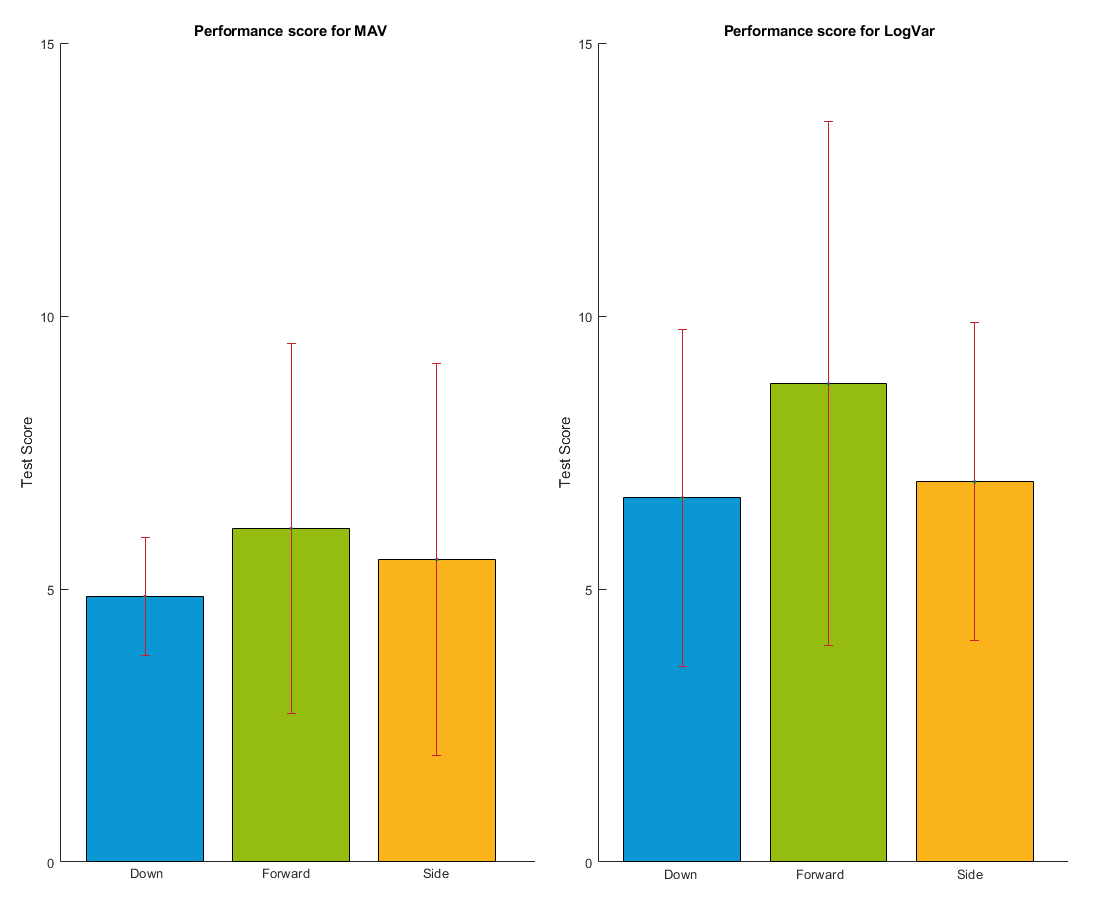
\includegraphics[width=0.4\textwidth]{figures/GotItTimeIMU}  %<--but is not needed.
		\caption{Plot of the actual data, red plot, superimposed on the output of the regressors trained with the MAV features. The plot is divided into four segments, where each segment shows a different movement performed. Each segment has the same sample size.}
		\label{fig:GotItTimeIMU}  %<--give the figure a label, so you can reference!
	\end{figure}
	
	\begin{table}[!thpb]
		\begin{center}
			\begin{tabular}{l l l}
				\hline
				\textbf{Limb position,feature} & \textbf{Overall mean error} & \textbf{Standard deviation}\\
				\hline
				Down, MAV & 4.8661 & $\pm 1.0839$ \\
				Forward, MAV & 6.1094 & $\pm 3.3852$ \\
				Side, MAV & 5.5442 & $\pm 3.5847$ \\
				Down, LogVar & 6.6691 & $\pm 3.0798$ \\
				Forward, LogVar & 8.7595 & $\pm 4.7969$ \\
				Side, LogVar & 6.9652 & $\pm 2.9144$ \\
				\hline
			\end{tabular}
			\caption{Test scores for the different limb for MAV and LogVar regressors with IMU included.}
		\end{center}
	\end{table}
	
	\begin{table}[!thpb]	
		\begin{center}
			\begin{tabular}{l l}
				\hline
				\textbf{Feature} & \textbf{P-Value}\\
				\hline
				MAV & 0.0319 \\
				LogVar & 0.4594 \\
				\hline
			\end{tabular}
			\caption{P-Values for comparison of the score in different limb positions with MAV and LogVar with IMU data included}
		\end{center}
	\end{table}
	
	The test with IMU data included shows a significant difference (p = 0.0319) between the test score in different limb positions for the MAV regressor with the worst performing position was with the arm pointed forward (mean = 6.1094), while there is no difference proven in the LogVar test (p = 0.4594).
	
	\begin{table}[!thpb]
		\begin{center}
			\begin{tabular}{l l l}
				\hline
				\textbf{Limb position,feature} & \textbf{Overall mean error} & \textbf{Standard deviation}\\
				\hline
				Down, MAV & 15.8889 & $\pm 0.3333$ \\
				Forward, MAV & 15.1111 & $\pm 2.3154$ \\
				Side, MAV & 15.5556 & $\pm 1.3333$ \\
				Down, LogVar & 14.7778 & $\pm 1.7159$ \\
				Forward, LogVar & 13.5556 & $\pm 2.1858$ \\
				Side, LogVar & 14.1111 & $\pm 1.8333$ \\
				\hline
			\end{tabular}
			\caption{RMSE for the implemented LogVar regressor}
		\end{center}
	\end{table}
	
	\begin{table}[!thpb]
		\begin{center}
			\begin{tabular}{l l}
				\hline
				\textbf{Compared Features} & \textbf{P-Value}\\
				\hline
				MAV & 0.2957 \\
				LogVar & 0.0037 \\
				\hline
			\end{tabular}
			\caption{P-Values for comparison of the number of targets reached in different limb positions with MAV and LogVar with IMU data included}
		\end{center}
	\end{table}
	
	The number of targets reached in the different limb positions can be proven to be significantly different (p = 0.0037) for the LogVar feature with IMU data included, where the lowest number of targets reached (mean = 13.5556) was found when the subjects pointed their arm forward. There was no significant difference found for the MAV regressor with IMU data included (p = 0.2957).
	
	\begin{figure}[!thpb]
		\centering
		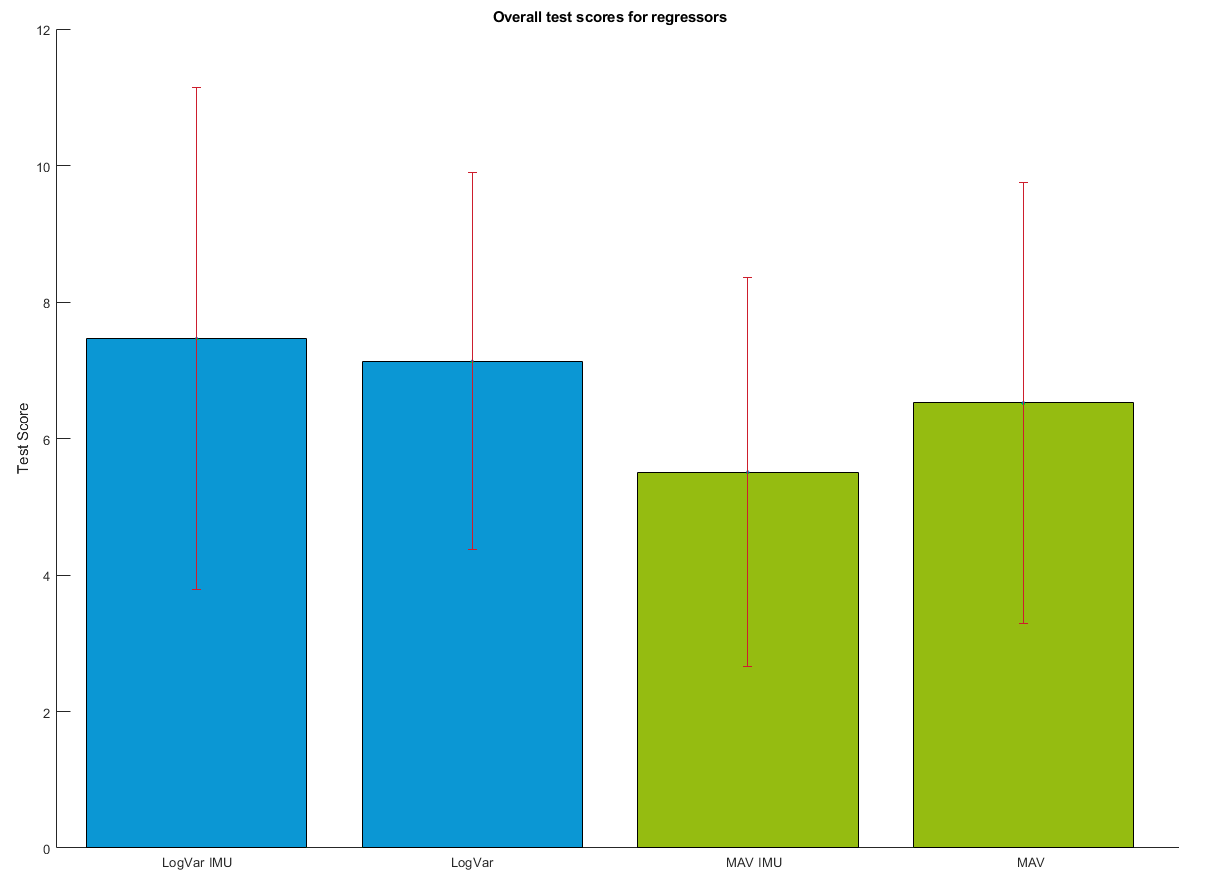
\includegraphics[width=0.4\textwidth]{figures/allRegressorBarzTimeScoreForTargetTest}  %<--but is not needed.
		\caption{Plot of the actual data, red plot, superimposed on the output of the regressors trained with the MAV features. The plot is divided into four segments, where each segment shows a different movement performed. Each segment has the same sample size.}
		\label{fig:TimeScoreTargets}  %<--give the figure a label, so you can reference!
	\end{figure}
	
	\begin{table}[!thpb]
		\begin{center}
			\begin{tabular}{l l l}
				\hline
				\textbf{Feature} & \textbf{Mean score} & \textbf{Standard deviation}\\
				\hline
				MAV & 6.5219 & $\pm 3.2253$ \\
				MAV w. IMU & 5.5066 & $\pm 2.8477$ \\
				LogVar & 7.1284 & $\pm 2.7619$ \\
				LogVar w. IMU & 7.4646 & $\pm 3.6740$ \\
				\hline
			\end{tabular}
			\caption{Average score of the target test for the four regressor designs}
		\end{center}
	\end{table}
	
	\begin{table}[!thpb]
		\begin{center}
			\begin{tabular}{l l}
				\hline
				\textbf{Compared features} & \textbf{P-Value}\\
				\hline
				LogVar w/ IMU, MAV w/ IMU & 0.5637 \\
				LogVar, MAV & 0.0833 \\
				LogVar w/ IMU, LogVar & 0.5637 \\
				MAV w/ IMU, MAV & 0.1779 \\
				\hline
			\end{tabular}
			\caption{P-Values for comparison of the overall scores of the target tests}
		\end{center}
	\end{table}
	
	When comparing all performance scores from the two feature trained regression control schemes without IMU, the Friedman's test proves no significant difference (LogVar: 7.1284 s, MAV: 6.5219 s; p = 0.0833). There is no significant difference to be found between LogVar and MAV with IMU data included (LogVar w/ IMU: 7.4646, MAV w/ IMU: 5.5066, p = 0.5637), and no difference was found between features with and without IMU for either MAV (w/o IMU: 6.5219, w/ IMU: 5.5066, p = 0.1779) or LogVar (w/o IMU: 7.1284, w/ IMU: 7.4646, p = 0.5637).
	
	\begin{figure}[!thpb]
		\centering
		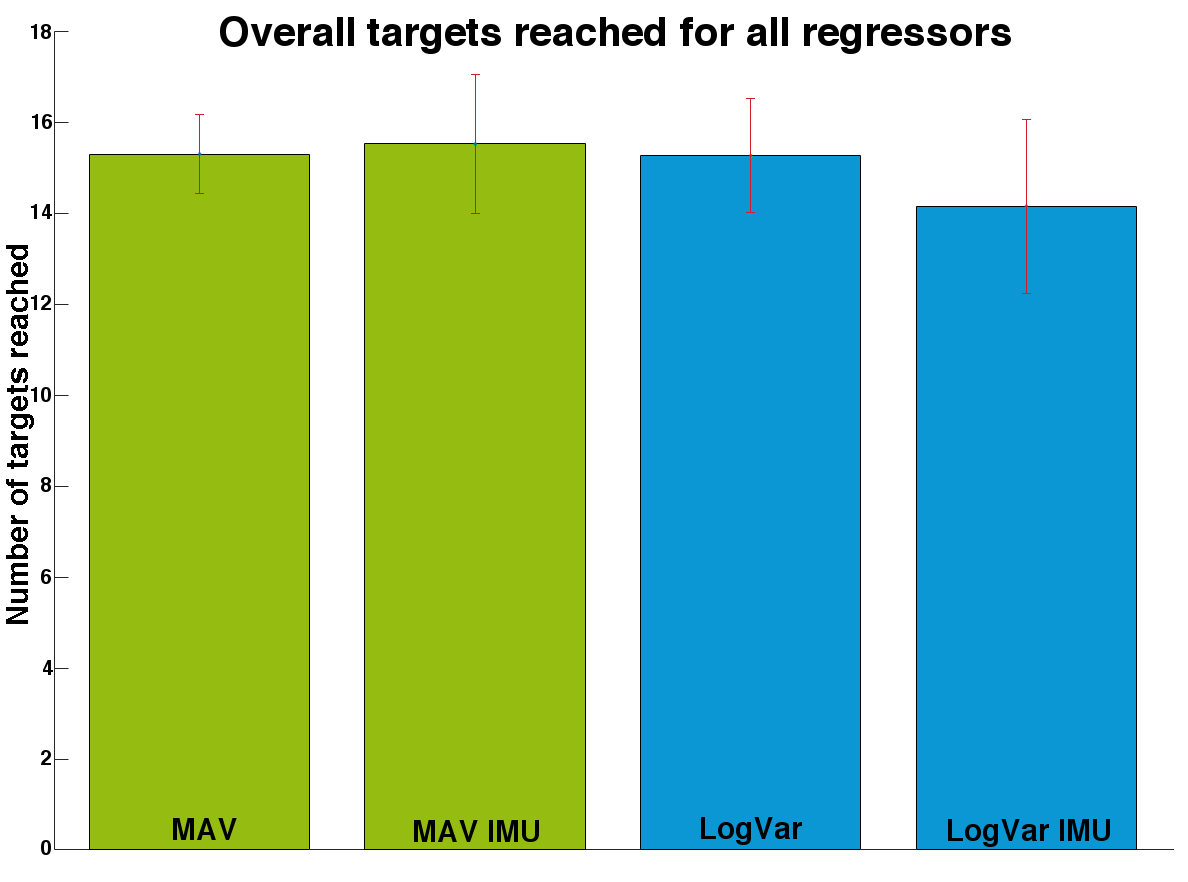
\includegraphics[width=0.4\textwidth]{figures/sumMoreBarsWithTargetsReachedForAllRegressors}  %<--but is not needed.
		\caption{Plot of the actual data, red plot, superimposed on the output of the regressors trained with the MAV features. The plot is divided into four segments, where each segment shows a different movement performed. Each segment has the same sample size.}
		\label{fig:TargetScoresTargets}  %<--give the figure a label, so you can reference!
	\end{figure}	
	
	\begin{table}[!thpb]
		\begin{center}
			\begin{tabular}{l l l}
				\hline
				\textbf{Feature} & \textbf{Overall mean error} & \textbf{Standard deviation}\\
				\hline
				MAV & 15.2963 & $\pm 0.8689$ \\
				MAV w/ IMU & 15.5185 & $\pm 1.5285$ \\
				LogVar & 15.2593 & $\pm 1.2586$ \\
				LogVar w/ IMU & 14.1481 & $\pm 1.9156$ \\
				\hline
			\end{tabular}
			\caption{Average number of targets reached in the target test for the four regressor designs}
		\end{center}
	\end{table}
	
	\begin{table}[!thpb]
		\begin{center}
			\begin{tabular}{l l}
				\hline
				\textbf{Compared Features} & \textbf{P-Value}\\
				\hline
				LogVar w/ IMU, MAV w/ IMU & 0.0017 \\
				LogVar, MAV & 1 \\
				LogVar w/ IMU, LogVar & 0.0016 \\
				MAV w/ IMU, MAV & 0.0124 \\
				\hline
			\end{tabular}
			\caption{P-Values for comparison targets reached in the target tests}
		\end{center}
	\end{table}
	
	A significant difference was found between LogVar and MAV when IMU was included (LogVar w/ IMU: 14.1481, MAV w/ IMU: 15.5185, p = 0.0017), and the same was found when including IMU data for both MAV (w/o IMU: 15.2963, w/ IMU: 15.5185, p = 0.0124) and LogVar (w/o IMU: 15.2593, w/ IMU: 14.1481, p = 0.0016). The performance was similar when comparing the overall number of targets reached for LogVar and MAV (p = 1).
	
	
	%	\subsection{Separability of the data} 
	
	
	
	%PCA performance for both features extracted is illustrated in Fig. \ref{PCA_MVA} (MVA) and in Fig. \ref{PCA_logvar} (logarithmic variance).
	%The importance of each component for MAV and logarithmic variance is represented in Fig. \ref{PCA_MVA}(a) and Fig. \ref{PCA_logvar}(a) respectively. On the one hand for the MAV feature making use of the three first components, 93.8\% of the data set can be described. On the other hand for the logarithmic variance feature the 93.97\% of the data set is describe with the three first components. This three PC have been plot for both features Fig. \ref{PCA_MVA}(b) and Fig. \ref{PCA_logvar}(b). There is no presence of remarkable outliers on two data sets and the formed clusters are easily distinguishable.
	
	
	%	\subsection{Regression accuracy} 
	
	%Through a quantitative examination of the figure(figure),is observed that MAV performed slightly better than the logarithmic variance for low intensities. However, both estimates yielded inaccurate fitting in high intensities, especially for ulnar deviation of the wrist. It has been extracted from the results illustrated in (figure), which represent the RMSE of the four different regressos for both features of the training data, than $RMSE_{MAV}$= 0.0867$\pm 0.031$ and $RMSE_{logvar}$= 0.1047$\pm 0.0273$. Overall MAV provided a lower mean but a higher standard deviation compared with logarithmic variance.
	
	%\begin{figure}[thpb]
	%\centering
	%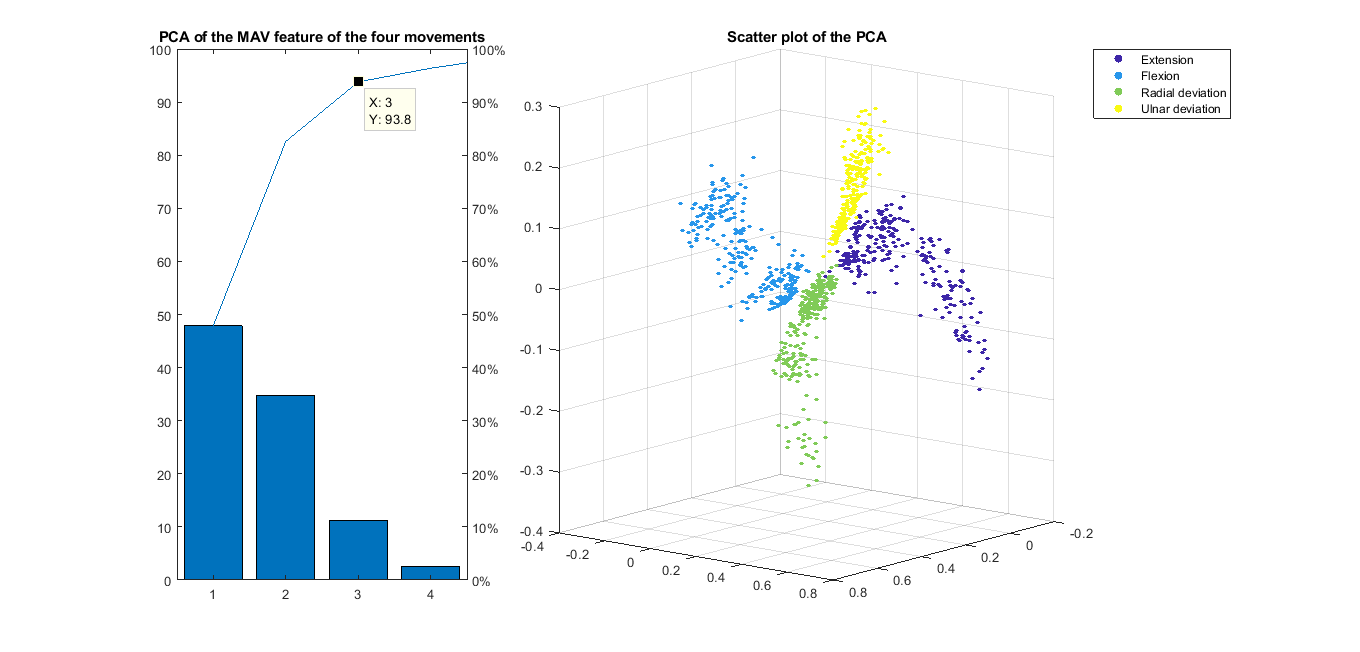
\includegraphics[scale=.27]{Figures/pcasubplotMAV}
	%\caption{Inductance of oscillation winding on amorphous
	%	magnetic core versus DC bias magnetic field}
	%\label{PCA_MVA}
	%\end{figure}
	
